%!TEX encoding = UTF-8 Unicode
%!TEX root = ../lect-w09.tex


\Subsection{\texttt{scala.collection}} %%%%%%%%%%%%%%%%%%%%%%%%%%%%%%%%%%%



% \begin{Slide}{Typparameter möjliggör generiska samlingar}\SlideFontSmall
%
% \begin{itemize}
%   \item Med \Emph{generisk} \Eng{generic} kod menar man att koden kan hantera data av \Alert{godtycklig} typ.
%   \item Funktioner och klasser kan, förutom vanliga parametrar, även ha \Emph{typparametrar} som skrivs i en \Alert{egen} parameterlista med \Alert{hakparenteser} i stället för vanliga parenteser.
%
%   \item En typparameter gör så att funktioner och datastrukturer blir \Emph{generiska}.
%
%   \item Exempel: Funktionerna \code{baklänges} 1--4 nedan är ordnade från specifik typ till mer generell typ.
%
% \begin{Code}
% def baklänges1(xs: Vector[Int]): Vector[Int] = xs.reverse
%
% def baklänges2[T](xs: Vector[T]): Vector[T] = xs.reverse
%
% def baklänges3(xs: Seq[T]): Vector[T] = xs.reverse.toVector
%
% def baklänges4(xs: Seq[T]): Seq[T] = xs.reverse  //reverse avgör samling
% \end{Code}
% \item Mer om typparametrar i w08.
% \end{itemize}
% \end{Slide}



\begin{Slide}{Hierarki av samlingstyper i \texttt{scala.collection} v2.13}

\begin{multicols}{2}
\begin{tikzpicture}[sibling distance=5.0em,->,>=stealth', inner sep=3pt, %scale=0.5,
  every node/.style = {shape=rectangle, draw, align=center,font=\small\ttfamily},
  class/.style = {fill=blue!20},
  trait/.style = {rounded corners, fill=red!20}]
  \node[trait] {Iterable}
      child { node[trait] {Seq} }
      child { node[trait] {Set} }
      child { node[trait] {Map} }
  ;
\end{tikzpicture}

\columnbreak

{\SlideFontTiny

\code{Iterable} har metoder som är implementerade med hjälp av: \\
\code{def foreach[U](f: Elem => U): Unit}\\
\code{def iterator: Iterator[A] }

}

\begin{itemize}\SlideFontTiny
\item[] \code{Seq}: ordnade i sekvens
\item[] \code{Set}: unika element
\item[] \code{Map}: par av (nyckel, värde)
\end{itemize}


\end{multicols}

{\SlideFontSmall Samlingen \Emph{\texttt{Vector}} är en \code{Seq} som är en \code{Iterable}. \\ \vspace{0.5em}%\pause
De konkreta samlingarna är uppdelade i dessa paket:\\
\code{scala.collection.immutable} \hfill där flera är \Emph{automatiskt} importerade\\
\code{scala.collection.mutable}  \hfill som \Alert{måste importeras} explicit\\%\pause
(undantag: primitiva förändringsbara \code{scala.Array} är automatiskt synlig)
}
\end{Slide}




\begin{Slide}{Metoden \texttt{iterator} ger en ''engångs-iterator''}\SlideFontSmall
Med \code{iterator} kan man iterera med \code{while}, men endast \Alert{en   gång}; sedan är iteratorn ''förbrukad''. (Men man kan be om en ny.) Används ''under huven'' i samlingsbiblioteket för att implementera andra metoder.
\begin{REPL}
scala> val xs = Vector(1,2,3,4)
val xs: Vector[Int] = Vector(1, 2, 3, 4)

scala> val it = xs.iterator
val it: Iterator[Int] = <iterator>

scala> while it.hasNext do print(it.next)
1234

scala> it.hasNext
val res0: Boolean = false

scala> it.next
java.util.NoSuchElementException: next on empty iterator
\end{REPL}
\Emph{Normalt} behöver man \Alert{inte} använda \code{iterator}: det finns oftast färdiga metoder som gör det man vill, till exempel \code{foreach}, \code{map}, \code{sum}, \code{min} etc.
\end{Slide}




% \ifkompendium
% \else
% \begin{Slide}{Hierarki av samlingar i scala.collection v2.12}\SlideFontTiny
% 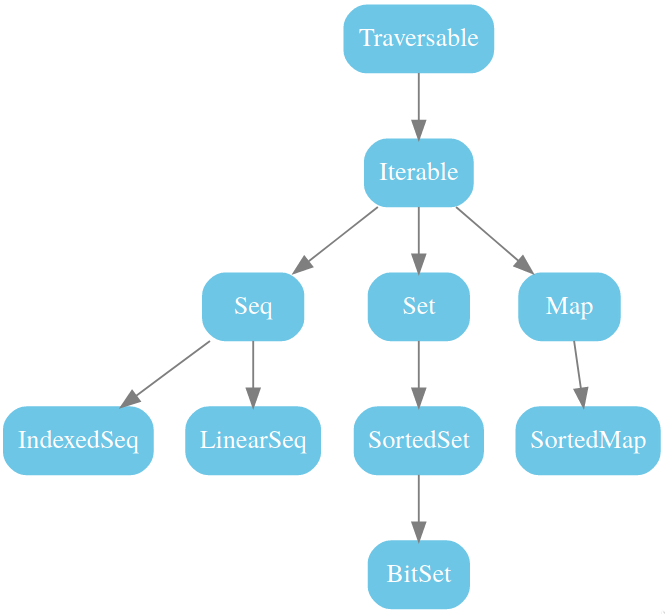
\includegraphics[width=0.6\textwidth]{../img/collection/collection-traits}\\
% %\noindent Läs mer om Scalas samlingar här: \\
% \url{https://docs.scala-lang.org/overviews/collections/overview.html}
% \end{Slide}
% \fi



\begin{Slide}{Mer specifika samlingstyper i \texttt{scala.collection}}
Det finns \Alert{mer specifika} \Emph{subtyper} av \code{Seq}, \code{Set} och \code{Map}:
\\ \vspace{1em}

\begin{tikzpicture}[sibling distance=5.8em,->,>=stealth', inner sep=3pt, %scale=0.5,
  every node/.style = {shape=rectangle, draw, align=center,font=\small\ttfamily},
  class/.style = {fill=blue!20},
  trait/.style = {rounded corners, fill=red!20}]
  \node[trait] {Iterable}
      child { node[trait, xshift=-2.4cm] {Seq}
        child { node[trait] {IndexedSeq} }
        child { node[trait] {LinearSeq} }
       }
      child { node[trait, yshift=-0.0cm] {Set}
        child { node[trait] {SortedSet} }
        child { node[trait] {BitSet} }
      }
      child { node[trait, xshift=1.0cm] {Map}
        child { node[trait] {SortedMap} }
    };
\end{tikzpicture}

\pause\vspace{0.5em}
\Emph{\texttt{Vector}} är en \Alert{\texttt{IndexedSeq}} medan
\Emph{\texttt{List}} är en \Alert{\texttt{LinearSeq}}.

\pause\vspace{1em}{\SlideFontSmall
\href
{https://docs.scala-lang.org/overviews/collections-2.13/overview.html}
{docs.scala-lang.org/overviews/collections-2.13/overview.html}
}
\end{Slide}

\begin{Slide}{Några oföränderliga och förändringsbara sekvenssamlingar}\SlideFontSmall
\begin{tabular}{r l l}
\texttt{scala.collection.\Emph{immutable}.Seq.} & & \\
 & \code|IndexedSeq.| & \\
 & & \Emph{\texttt{Vector}} \\
 & & \Emph{\texttt{Range}} \\
 & \code|LinearSeq.| & \\
 & & \Emph{\texttt{List}} \\
   & & \Emph{\texttt{Queue}} \\

\texttt{scala.collection.\Alert{mutable}.Seq.} & & \\
 & \code|IndexedSeq.| & \\
 & & \Alert{\texttt{ArrayBuffer}} \\
 & & \Alert{\texttt{StringBuilder}} \\
 & \code|LinearSeq.| & \\
 & & \Alert{\texttt{ListBuffer}} \\
   & & \Alert{\texttt{Queue}} \\
\end{tabular}

{\SlideFontTiny Fördjupning: Studera samlingars prestanda-egenskaper här:\\ \href{https://docs.scala-lang.org/overviews/collections-2.13/performance-characteristics.html}{docs.scala-lang.org/overviews/collections-2.13/performance-characteristics.html}}
\end{Slide}



\begin{Slide}{Några användbara metoder på samlingar}\SlideFontTiny
\begin{tabular}{r r l}\hline
\texttt{\Emph{Iterable}}
  & \code|xs.size| & antal elementet \\
  & \code|xs.head| & första elementet \\
  & \code|xs.last| & sista elementet \\
  & \code|xs.take(n)| & ny samling med de första n elementet \\
  & \code|xs.drop(n)| & ny samling utan de första n elementet \\
  & \code|xs.foreach(f)| & gör \code|f| på alla element, returtyp \code|Unit|\\
  & \code|xs.map(f)| & gör \code|f| på alla element, ger ny samling \\
  & \code|xs.filter(p)| & ny samling med bara de element där p är sant\\
  & \code|xs.groupBy(f)| & ger en \code|Map| som grupperar värdena enligt f\\
  & \code|xs.mkString(",")| & en kommaseparerad sträng med alla element\\ 
  & \code|xs.zip(ys)| & ny samling med par (x, y); ''zippa ihop'' xs och ys \\
  & \code|xs.zipWithIndex| & ger en \code|Map| med par (x, index för x) \\
  & \code|xs.sliding(n)| & ny samling av samlingar genom glidande ''fönster''\\ \hline

\texttt{\Emph{Seq}}
  & \code|xs.length| & samma som \code|xs.size| \\
  & \code|xs :+ x| & ny samling med x sist efter xs \\
  & \code|x +: xs| & ny samling med x före xs \\ \hline

\end{tabular}
Prova fler samlingsmetoder ur snabbreferensen: ~~\url{http://cs.lth.se/quickref}

\vspace{0.5em}\Emph{Minnesregel} för \code{+:} och \code{:+  } \Alert{Colon on the collection side}

\end{Slide}



% \ifkompendium\else

% \begin{Slide}{scala.collection.immutable}
% 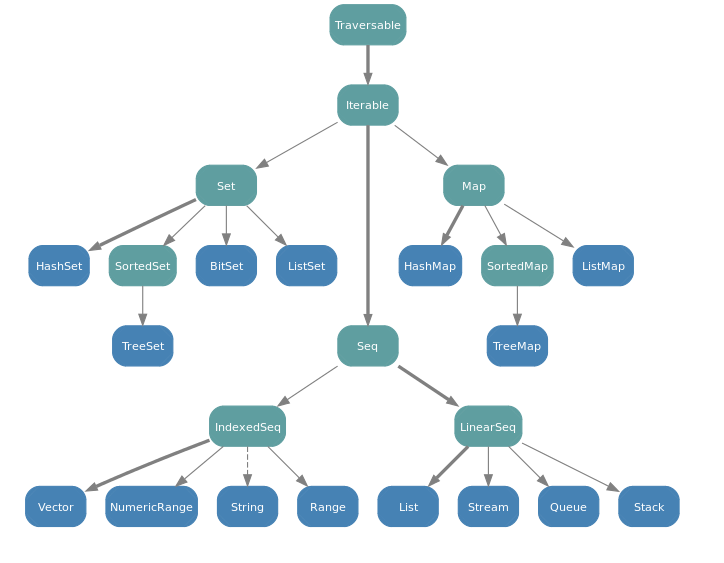
\includegraphics[width=0.67\textwidth]{../img/collection/collection-immutable}~~%
% 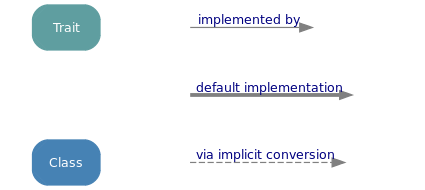
\includegraphics[width=0.3\textwidth]{../img/collection/collection-legend}
% \end{Slide}


% \begin{Slide}{scala.collection.mutable}
% 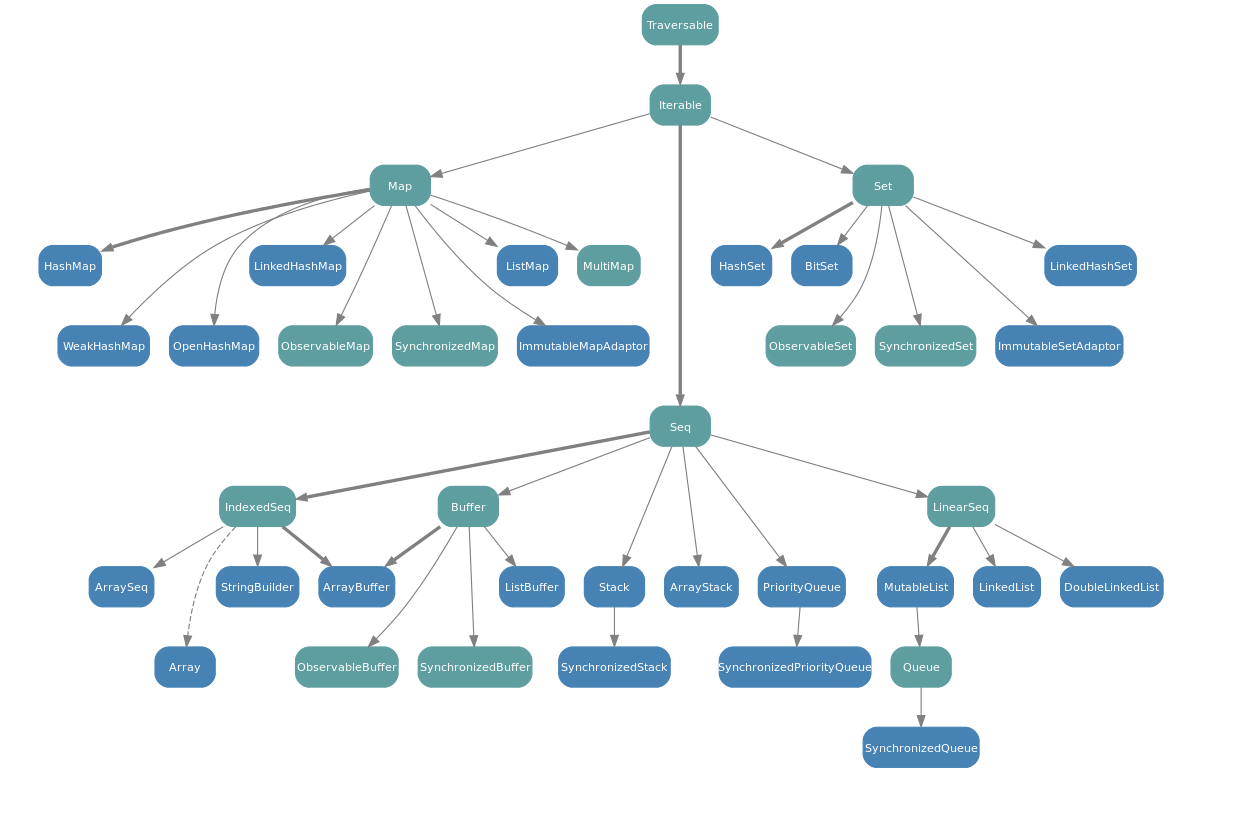
\includegraphics[width=1.05\textwidth]{../img/collection/collection-mutable}
% \end{Slide}

% \fi



% \begin{Slide}{\texttt{Vector} eller \texttt{List}?}\SlideFontTiny
% {\href{http://stackoverflow.com/questions/6928327/when-should-i-choose-vector-in-scala}{stackoverflow.com/questions/6928327/when-should-i-choose-vector-in-scala}}
%
% \begin{enumerate}
% \item If we only need to transform sequences by operations like map, filter, fold etc: basically it does not matter, we should program our algorithm generically and might even benefit from accepting parallel sequences. For sequential operations List is probably a bit faster. But you should benchmark it if you have to optimize.
%
% \item If we need a lot of random access and different updates, so we should use vector, list will be prohibitively slow.
%
% \item If we operate on lists in a classical functional way, building them by prepending and iterating by recursive decomposition: use list, vector will be slower by a factor 10-100 or more.
%
% \item If we have an performance critical algorithm that is basically imperative and does a lot of random access on a list, something like in place quick-sort: use an imperative data structure, e.g. ArrayBuffer, locally and copy your data from and to it.
% \end{enumerate}
% {\href{http://stackoverflow.com/questions/20612729/how-does-scalas-vector-work}{stackoverflow.com/questions/20612729/how-does-scalas-vector-work}}\\
% Mer om tids- och minneskomplexitet i fördjupningskursen och senare kurser.
% \end{Slide}








\Subsection{Repetition: sekvens}

\begin{Slide}{Repetition: Vad är en sekvens?}
\begin{itemize}
\item En sekvens är en \Emph{följd av element} som
  \begin{itemize}
   \item är \Alert{numrerade} (t.ex. från noll), och
   \item är av en viss \Alert{typ} (t.ex. heltal).
  \end{itemize}
  \pause
\item En sekvens kan innehålla \Alert{dubbletter}.
\item En sekvens kan vara \Alert{tom} och ha längden noll.
\item Exempel på en icke-tom sekvens med dubbletter:
\begin{REPLnonum}
scala> val xs = Vector(42, 0, 42, -9, 0, 13, 7)
val xs: Vector[Int] = Vector(42, 0, 42, -9, 0, 13, 7)
\end{REPLnonum}
\pause
\item \Emph{Indexering} ger ett element via dess ordningsnummer:
\begin{REPL}
scala> xs(2)
val res0: Int = 42

scala> xs.apply(2)
val res1: Int = 42
\end{REPL}
\end{itemize}
\end{Slide}


\begin{Slide}{En sträng är också en \texttt{IndexedSeq[Char]}}\SlideFontSmall
Det sker vid behov \Emph{implicit konvertering} från \code{String} till \code{IndexedSeq[Char]}.
\begin{REPLnonum}
scala> val x: IndexedSeq[Char] = "hej"
val x: IndexedSeq[Char] = hej
\end{REPLnonum}

Detta gör att \Alert{alla samlingsmetoder på \texttt{Seq} även funkar på strängar} och även flera andra smidiga strängmetoder erbjuds \Alert{utöver} de som finns i \href{https://www.scala-lang.org/api/current/scala/collection/StringOps.html}{\code{java.lang.String}} genom klassen \href{http://www.scala-lang.org/api/current/scala/collection/immutable/StringOps.html}{\code{StringOps}}.

\vspace{0.5em}
\begin{REPLnonum}
scala> "hej".  //tryck på TAB och se alla strängmetoder
JLine: do you wish to see all 248 possibilities (42 lines)?
\end{REPLnonum}
Detta är en stor fördel med Scala jämfört med många andra språk, som har strängar som inte kan allt som andra sekvenssamlingar kan.
\end{Slide}
  

\begin{Slide}{Konvertera mellan olika samlingstyper}
\begin{itemize}
\item För vanligt förekommande konverteringar finns metoderna \code{toVector}, \code{toList},  \code{toArray}, \code{toBuffer}, \code{toMap}, \code{toSeq}, \code{toIndexedSeq}, \code{toSet},  \code{toString}
\item Metoden \texttt{to} (ny från Scala 2.13) tar ett \Emph{kompanjonsobjekt} ur samlingsbiblioteket som argument och kan användas för konvertering till godtycklig samlingstyp.
\item Detta kräver kopiering om underliggande representation är olika och samlingen är förändringsbar.
\item Kan användas för att t.ex. konvertera mellan oföränderlig och förändringsbar samling:
\end{itemize}
\begin{REPLnonum}
scala> val ms = Set(1,2,3).to(collection.mutable.Set)
val ms: scala.collection.mutable.Set[Int] = HashSet(1, 2, 3)
\end{REPLnonum}
\end{Slide}


\Subsection{Mängd} %%%%%%%%%%%%%%%%%%%%%%%%%%%%%%%%%%%%%%%%%%%%%%%%%%%%%%


\begin{Slide}{Vad är en mängd?}\SlideFontSmall
\begin{itemize}
\item En \Emph{mängd} är en samling \Alert{unika} element av en viss \Alert{typ}.
\item En mängd kan alltså inte innehålla dubbletter:
\begin{REPLnonum}
scala> Set(1,1,2,2,3,3,4,4,5,5)
val res0: Set[Int] = HashSet(5, 1, 2, 3, 4)
\end{REPLnonum}
\pause
\item En mängd är \Alert{inte}  en sekvens: du kan inte utgå från att elementen ligger i någon viss ordning, t.ex. den ordning som de ges vid konstruktion; en mängd har ej längd, men en \Emph{storlek}; metoden \code{size} ger antalet element men metoden \code{length} saknas.
\item En mängd kan vara \Alert{tom} och har då storleken \code{0}.
\pause
\item Man kan gå igenom element i \Emph{någon} ordning (exakt vilken är ej def.), med till exempel \code{xs.map(f)} eller \code{for (x <- xs) yield f(x)}
\pause
\item Det går \Alert{inte} att indexera i en mängd med \code{apply}, som i stället ger \Emph{innehållstest}: \code{Set(1,2,3).apply(3) == true}
\item En mängd \code{Set[T]} med element av typen \code{T} kan således ses som ett \Emph{predikat för innehållstest}: alltså en funktion \code{T => Boolean} som är \code{true} om elementet finns annars \code{false}
\end{itemize}
\end{Slide}


\begin{Slide}{Exempel: Oföränderlig mängd}
\setlength{\leftmargini}{1em}
\begin{itemize}
\item \Emph{Skapa}:
\begin{REPLnonum}
scala> var xs = Set("gurka", "tomat", "banan", "pingvin")
\end{REPLnonum}

\item \Emph{Läsa}: avgöra medlemskap
\begin{REPLnonum}
scala> xs("gurka")
val res1: Boolean = true
\end{REPLnonum}

\item \Emph{Uppdatera}: lägg till element (händer inget om redan finns)
\begin{REPLnonum}
scala> xs = xs + "jordekorre"
\end{REPLnonum}

\item \Emph{Ta bort}: (om finns, annars händer inget)
\begin{REPLnonum}
scala> xs = xs - "gurka"
\end{REPLnonum}
\end{itemize}
{\SlideFontTiny\code{SLUT} = Skapa, Läsa, Uppdatera, Ta bort \hfill\code{CRUD} = Create, Read, Update, Delete}
\end{Slide}


\begin{Slide}{Mysteriet med de försvunna elementen}
Vad händer här?
\begin{REPLnonum}
scala> val xs1 = Vector(1,2,3,4,5,6)
scala> xs1.map(_ % 2).count(_ == 0)
val res0: Int = 3                          // antalet jämna tal
scala> val xs2 = Set(1,2,3,4,5,6)
scala> xs2.map(_ % 2).count(_ == 0)
val res1: Int = 1                          // varför?
\end{REPLnonum}
\pause
Mängdegenskaper ger att \code{xs2.map(_ % 2) == Set(0, 1)}\\
Fundera alltid noga på om du \Alert{riskerar att förlora duplikat} som du egentligen hade velat behålla!\\
\pause
Använd \code{toSeq} på mängd om du behöver sekvensegenskaper:
\begin{REPLnonum}
scala> xs2.toSeq.map(_ % 2).count(_ == 0)
val res1: Int = 3         // med toSeq blir det som vi ville
\end{REPLnonum}

\end{Slide}
  
  




\begin{Slide}{Exempel: Förändringsbar mängd}\SlideFontSmall
Med en \Alert{förändringsbar} mängd kan man stegvis utöka på plats.
\begin{REPL}
scala> val mängd = scala.collection.mutable.Set.empty[Int]

scala> for i <- 1 to 1_000_000 do mängd += i

scala> mängd.contains(-1)   // samma som mängd(-1) eller mängd.apply(-1)
\end{REPL}
En \Emph{mängd} är \Alert{snabb} på att avgöra om ett element \Alert{finns eller inte} i mängden. Ingen linjärsökning krävs eftersom den smarta implementationen av datastrukturen medger snabb uppslagning \Eng{lookup} av ett element.
\pause
\\\vspace{0.5em}Men i en sekvens krävs linjärsökning vid innehållstest:
\begin{REPL}
scala> val sekvens = (1 to 1_000_000).toVector

scala> sekvens.contains(-1)   // kräver linjärsökning ända till slutet
\end{REPL}
\pause\SlideFontTiny Övning: Testa själv att mäta tidsskillnaden med hjälp av:
\begin{Code}
def nanos(b: => Unit) = { val t0 = System.nanoTime; b; System.nanoTime - t0 }
\end{Code}

\end{Slide}






\Subsection{Nyckel-värde-tabell} %%%%%%%%%%%%%%%%%%%%%%%%%%%%%%%%%%%%%%%%


\begin{Slide}{Vad är en nyckel-värde-tabell?}\SlideFontSmall
\begin{itemize}
\item En \Emph{nyckel-värde-tabell} är en samling element som är \Alert{par} med:\\
en \Emph{nyckel} av någon typ \code{K} och ett \Emph{värde} av någon typ \code{V}.
\item En sådan tabell kan skapas ur en sekvens av par \code{(k, v)}\\
där \code{k} är en nyckel och \code{v} är ett värde:
\begin{REPL}
scala> val ålder = Map("Björn" -> 42, "Sandra" -> 35, "Kim" -> 19)
val ålder: Map[String, Int] = Map(Björn -> 42, Sandra -> 35, Kim -> 19)
\end{REPL}
\item Tabellens nycklar utgör en mängd som ges av metoden \code{keySet};\\
nycklarna är \Alert{unika}.
\item Elementen utgör \Alert{inte en sekvens} och har ingen speciell ordning;
\\en nyckel-värde-tabell har ej längd, men en \Emph{storlek};\\metoden \code{size} ger antalet element.
\pause
\item En tabell kan ses som en uppslagsfunktion \Eng{dictionary}:\\alltså en funktion \code{K => V} som ger ett värde givet en nyckel.
\end{itemize}
\end{Slide}


\begin{Slide}{Den fantastiska nyckel-värde-tabellen \texttt{Map}}\SlideFontSmall
\begin{itemize}
\item En \Emph{nyckel-värde-tabell} \Eng{key-value table} är en slags generaliserad vektor där man kan ''indexera'' med godtycklig typ.

\item Kallas även \href{https://sv.wikipedia.org/wiki/Hashtabell}{\Emph{hashtabell}} \Eng{hash table}, \Emph{lexikon} \Eng{Dictionary} eller \Emph{mapp} \Eng{Map} (det blir lätt sammanblandning med metoden \code{map}).

\item Om man vet nyckeln kan man slå upp värdet \Alert{snabbt}, på liknande sätt som indexering sker i en vektor givet heltalsindex.

\item Denna datastruktur är \Alert{mycket användbar} och fungerar som en slags databas i kombination med filtrering, registrering, etc.
\end{itemize}
\end{Slide}


\begin{Slide}{Exempel: Oföränderlig nyckel-värde-tabell}
\setlength{\leftmargini}{1em}
\begin{itemize}
\item \Emph{Skapa}: ge par till metoden \code{apply} 
\begin{REPLsmall}
scala> var födelse = Map("C" -> 1972,  "C++" -> 1983, "C#" -> 2000,
  "Scala" -> 2004, "Java" -> 1995, "Javascript" -> 1995, "Python" -> 1991)
\end{REPLsmall}

\item \Emph{Läsa}: slå upp ett värde med hjälp av en nyckel
\begin{REPLsmall}
scala> val year = födelse.apply("Scala")
val year: Int = 2004
\end{REPLsmall}

\item \Emph{Uppdatera}: lägga till ett par, ersätta ett par
\begin{REPLsmall}
scala> födelse = födelse + ("Kotlin" -> 2011)
födelse: Map[String, Int] = HashMap(Scala -> 2004, C# -> 2000, Python -> 1991, 
Javascript -> 1995, C -> 1972, C++ -> 1983, Kotlin -> 2011, Java -> 1995)
\end{REPLsmall}

\item \Emph{Ta bort} ett par via nyckeln (om finns, annars händer inget)
\begin{REPLsmall}
scala> födelse = födelse - "Python"
födelse: Map[String, Int] = HashMap(Scala -> 2004, C# -> 2000, 
Javascript -> 1995, C -> 1972, C++ -> 1983, Kotlin -> 2011, Java -> 1995)
\end{REPLsmall}
\end{itemize}
\end{Slide}


\begin{Slide}{Fler exempel nyckel-värde-tabell}\SlideFontSmall
Några ofta förekommande metoder på tabeller:
\begin{itemize}
\item \code{xs.keySet} ger en mängd av alla nycklar
\item \code{xs.map(f)} mappar funktionen f på alla par av (key, value)
\item \code{xs.map((k, v) => k -> f(v))} mappar funktionen f på alla värden
\end{itemize}
\begin{REPLsmall}
scala> val färg = Map("gurka" -> "grön", "tomat"->"röd", "aubergine"->"lila")
val färg: Map[String, String] = 
  Map(gurka -> grön, tomat -> röd, aubergine -> lila)

scala> färg("gurka")
val res0: String = grön

scala> färg.keySet
val res1: Set[String] = Set(gurka, tomat, aubergine)

scala> val ärGrönSak = färg.map((k,v) => (k, v == "grön"))
val ärGrönSak: Map[String,Boolean] = 
  Map(gurka -> true, tomat -> false, aubergine -> false)

scala> val baklängesFärg = färg.map((k, v) => k -> v.reverse)
val baklängesFärg: Map[String,String] = 
  Map(gurka -> nörg, tomat -> dör, aubergine -> alil)
\end{REPLsmall}

\end{Slide}



\begin{Slide}{Från sekvens av par till tabell}
\begin{REPL}
scala> val xs = Vector(("Kim",42), ("Pam", 42), ("Kim", 50), ("Pam", 50))
val xs: Vector[(String, Int)] = 
  Vector((Kim,42), (Pam,42), (Kim,50), (Pam,50))

scala> xs.toMap
val res0: Map[String, Int] = 
  Map(Kim -> 50, Pam -> 50) // inga dublettnycklar

scala> val grupperaEfterNamn = xs.groupBy(_._1)
grupperaEfterNamn: Map[String,Vector[(String, Int)]] =
  Map(Kim -> Vector((Kim,42), (Kim,50)), Pam -> Vector((Pam,42), (Pam,50)))

scala> val grupperaEfterÅlder = xs.groupBy(_._2)
grupperaEfterÅlder: Map[Int,Vector[(String, Int)]] =
  Map(50 -> Vector((Kim,50), (Pam,50)), 42 -> Vector((Kim,42), (Pam,42)))
\end{REPL}
\end{Slide}
  
  
\begin{Slide}{Övning: Implementera en \texttt{Multimap}}
\begin{itemize}
\item En \Emph{multimap} är en speciell nyckel-värde-tabell där värdena utgör en samling (ofta en mängd).
\item En multimap samlar alla värden som har samma nyckel.
\item Om du lägger till ett värde så ersätts inte värdet; i stället utökas samlingen av värden.
\end{itemize}
\begin{REPL}
scala> val m = Map(1 -> 2, 1 -> 3, 2 -> 1, 2 -> 2)  // senaste värdet gäller
val m: Map[Int, Int] = Map(1 -> 3, 2 -> 2)

scala> val mm = Multimap(1 -> 2, 1 -> 3, 2 -> 1, 2 -> 2)  // värdena samlas
val mm: Multimap[Int, Int] = Multimap(1 -> Set(2, 3), 2 -> Set(1, 2))
\end{REPL}
Övning: Implementera en multimap som fungerar som ovan, med hjälp av en case-klass med attributet \code{toMap} som är en oföränderlig nyckel-värde-tabell där värdena är en mängd. \\Tips: Använd~\code{groupBy}
\end{Slide}

\begin{Slide}{Lösning: \texttt{Multimap}}
\begin{CodeSmall}
case class Multimap[K, V] private (toMap: Map[K,Set[V]]):
  def apply(k: K): Set[V] = toMap(k)
  
  def +(kv: (K, V)): Multimap[K, V] = kv match 
    case (k, v) if toMap.isDefinedAt(k) => Multimap(toMap.updated(k, toMap(k) + v))
    case (k, v) => Multimap(toMap + (k -> Set(v)))
  
  override def toString = toMap.mkString("Multimap(",", ",")")

object Multimap:
  def apply[K, V](kvs: (K,V)*): Multimap[K, V] = 
    new Multimap(kvs.groupBy(_._1).map((k,xs) => k -> xs.map(_._2).toSet))
\end{CodeSmall}
\end{Slide}


\Subsection{Tips inför veckans uppgifter}

\begin{Slide}{Speciella metoder på förändringsbara samlingar}\SlideFontSmall
Både \code{Set} och \code{Map} finns i \Alert{förändringsbara} varianter med extra metoder för uppdatering av innehållet ''på plats'' utan att nya samlingar skapas.
\begin{REPL}
scala> import scala.collection.mutable

scala> val ms = mutable.Set.empty[Int]
val ms: scala.collection.mutable.Set[Int] = HashSet()

scala> ms += 42
val res0: scala.collection.mutable.Set[Int] = HashSet(42)

scala> ms ++= Seq(1, 2, 3, 1, 2, 3)  // metoden ++= gör samma som addAll 
val res1: scala.collection.mutable.Set[Int] = HashSet(1, 2, 3, 42)

scala> (ms diff Set(1)).mkString("Mängd: ", ", ", " Antal: " + ms.size)
val res2: String = Mängd: 2, 3, 42 Antal: 4

scala> val ordpar = mutable.Map.empty[String, String]
scala> ordpar ++= Seq("hej" -> "svejs", "abra" -> "kadabra", "ada" -> "lovelace")
scala> println(ordpar("abra"))
kadabra
\end{REPL}
\end{Slide}


\begin{Slide}{Övning: Förändringsbar lokalt, returnera oföränderlig}
\SlideFontSmall
Om du vill implementera en imperativ algoritm med en föränderlig samling:\\
Gör gärna detta \Alert{lokalt} i en \Alert{förändringsbar} samling och returnera sedan en \Emph{oföränderlig} samling, genom att köra t.ex. \code{toSet} på en mängd, eller \code{toMap} på en hashtabell, eller \code{toVector} på en \code{ArrayBuffer} eller \code{Array}.\\~\\
Exempel där lösningen har nytta av lokal förändring på plats:
\begin{Code}
def kastaTärningTillsAllaUtfallUtomEtt(sidor: Int = 6): (Int, Set[Int]) = ???
\end{Code}
\begin{REPL}
scala> kastaTärningTillsAllaUtfallUtomEtt()
val res0: (Int, Set[Int]) = (13,HashSet(5, 1, 6, 2, 3))
\end{REPL}
\end{Slide}


\begin{Slide}{Övning: Förändringsbar lokalt, returnera oföränderlig}
\SlideFontSmall
Om du vill implementera en imperativ algoritm med en föränderlig samling:\\
Gör gärna detta \Alert{lokalt} i en \Alert{förändringsbar} samling och returnera sedan en \Emph{oföränderlig} samling, genom att köra t.ex. \code{toSet} på en mängd, eller \code{toMap} på en hashtabell, eller \code{toVector} på en \code{ArrayBuffer} eller \code{Array}.
\begin{Code}
def kastaTärningTillsAllaUtfallUtomEtt(sidor: Int = 6): (Int, Set[Int]) = 
  /* 
    låt s vara en tom förändringsbar heltalsmängd
    låt n vara noll
    så länge mängden s är mindre än sidor - 1 gör:
      lägg till ett nytt tärningskast i s
      uppdatera n så att vi räknar hur många slumptal som dragits
  */
  (n, s.toSet)   // notera toSet som ger oföränderlig mängd
\end{Code}
\begin{REPL}
scala> kastaTärningTillsAllaUtfallUtomEtt()
val res0: (Int, Set[Int]) = (13,HashSet(5, 1, 6, 2, 3))
\end{REPL}
\end{Slide}


\begin{Slide}{Lösning: Förändringsbar lokalt, returnera oföränderlig}
\SlideFontSmall
Om du vill implementera en imperativ algoritm med en föränderlig samling:\\
Gör gärna detta \Alert{lokalt} i en \Alert{förändringsbar} samling och returnera sedan en \Emph{oföränderlig} samling, genom att köra t.ex. \code{toSet} på en mängd, eller \code{toMap} på en hashtabell, eller \code{toVector} på en \code{ArrayBuffer} eller \code{Array}.
\begin{Code}
def kastaTärningTillsAllaUtfallUtomEtt(sidor: Int = 6): (Int, Set[Int]) = 
  val s = scala.collection.mutable.Set.empty[Int] //förändringsbar lokalt
  var n = 0
  while s.size < sidor - 1 do
    s += util.Random.nextInt(sidor) + 1 
    n += 1
  (n, s.toSet)   // notera toSet som ger oföränderlig mängd
\end{Code}
\begin{REPL}
scala> kastaTärningTillsAllaUtfallUtomEtt()
val res0: (Int, Set[Int]) = (13,HashSet(5, 1, 6, 2, 3))
\end{REPL}
I veckans uppgifter används detta i en s.k. \Emph{builder}: Först bygga upp en förändringsbar struktur i \code{FreqMapBuilder} steg för steg,  
och sedan, då alla tillägg är gjorda, övergå till oföränderlig struktur \code{Map[String, Int]}. 
\end{Slide}


\begin{Slide}{Metoden \texttt{sliding}}\SlideFontSmall
Metoden \code{sliding(n)} skapar med ett ''glidande fönster'' en sekvens av
delsekvenser av längd \code{n} genom att ''svepa fönstret'' från början till slut:
\begin{REPL}
scala> val xs = "fem myror är fler än fyra elefanter".split(' ').toVector
val xs: Vector[String] = Vector(fem, myror, är, fler, än, fyra, elefanter)

scala> xs.sliding(2).toVector
val res0: Vector[Vector[String]] =
  Vector(Vector(fem, myror), Vector(myror, är), Vector(är, fler),
      Vector(fler, än), Vector(än, fyra), Vector(fyra, elefanter))

scala> xs.sliding(3).toVector
val res1: Vector[Vector[String]] =
  Vector(Vector(fem, myror, är), Vector(myror, är, fler),
    Vector(är, fler, än), Vector(fler, än, fyra),
      Vector(än, fyra, elefanter))
\end{REPL}
Denna metod har du nytta av på veckans laboration!
\\(se fler exempel på övning)
\end{Slide}
  
  

\begin{Slide}{Metoderna zipWithIndex, groupBy}
\vspace{-0.5em}
\begin{REPL}
scala> val kort = Vector("Knekt", "Dam", "Kung", "Äss")

scala> val kortIndex = kort.zipWithIndex.toMap
kortIndex: Map[String,Int] = Map(Knekt -> 0, Dam -> 1, Kung -> 2, Äss -> 3)

scala> kortIndex("Kung") > kortIndex("Knekt")
res0: Boolean = true

scala> kortIndex.map(p => p._1 -> (p._2 + 11))

scala> val tärningskast = Vector(1,2,3,4,5,6,2,4,6)

scala> val grupperaStörreÄnFyra = tärningskast.groupBy(_ > 4)
grupperaStörreÄnFyra: Map[Boolean,Vector[Int]] =
  Map(false -> Vector(1, 2, 3, 4, 2, 4), true -> Vector(5, 6, 6))

scala> val grupperaLika = tärningskast.groupBy(x => x)
grupperaLika: Map[Int,Vector[Int]] = Map(5 -> Vector(5), 1 -> Vector(1),
  6 -> Vector(6, 6), 2 -> Vector(2, 2), 3 -> Vector(3), 4 -> Vector(4, 4))

scala> val frekvens = tärningskast.groupBy(x => x).map((k,v) => k -> v.size)
frekvens: Map[Int,Int] = Map(5 -> 1, 1 -> 1, 6 -> 2, 2 -> 2, 3 -> 1, 4 -> 2)

\end{REPL}
\end{Slide}

\begin{Slide}{Fler användbara samlingsmetoder}
Exempel att öva på: räkna bokstäver i ord.  \\
Undersök vad som händer i REPL:
\begin{Code}[basicstyle=\SlideFontSize{9}{13}\ttfamily]
val ord = "sex laxar i en laxask sju sjösjuka sjömän"
val uppdelad = ord.split(' ').toVector
val ordlängd = uppdelad.map(_.length)
val ordlängdMap = uppdelad.map(s => (s, s.size)).toMap
val grupperaEfterFörstaBokstav = uppdelad.groupBy(s => s(0))
val bokstäver = ord.toVector.filter(_ != ' ')
val antalX = bokstäver.count(_ == 'x')
val grupperade = bokstäver.groupBy(ch => ch)
val antal = grupperade.map(p => p._1 -> p._2.size)
//samma som ovan men utnyttjar "parameter untupling":
val antal2 = grupperade.map((k,v) => k -> v.size) 
val sorterat = antal.toVector.sortBy(_._2)
val vanligast = antal.maxBy(_._2)
\end{Code}
%https://dotty.epfl.ch/docs/reference/other-new-features/parameter-untupling.html
\end{Slide}
    
    
